%! TEX root = main.tex
\documentclass[main.tex]{subfiles}
\begin{document}
\section{Einführung in den 3D-Druck}
Der 3D-Druck, auch bekannt als Additive Manufacturing (AM) oder Rapid Prototyping ist ein bereits lange bekanntes Forschungsfeld, da bereits im Jahr 1986 das erste Verfahren, SLA (Stereolithographie), von Charles Hull entwickelt wurde. Jedoch basierten diese frühen Methoden allesamt auf der Verarbeitung von Polymeren in diversen Formen, zum Beispiel bediente sich SLA einem UV-reaktiven Kunstharz. Das wohl bekannteste Verfahren ist FDM (Filament-Deposition-Modelling), welches im Gegensatz zu SLA mit Spulen an Filament (meist $D=\qty{1.75}{mm}$) arbeitet. Dieses Filament besteht aus thermoplastischen Polymeren, das heißt der Polymer kann aufgeschmolzen werden und wird daraufhin durch eine Düse aufgetragen. Dieser Vorgang ist im Konstrast zu SLA reversibel, da ein Thermoplast immer wieder aufgeschmolzen werden kann.\parencite{BHATIA20231060} Das Kunstharz jedoch wird wenn der Photopolymer ausreagiert hat nie wieder in seinen urspünglichen Zustand zurückführbar sein.\parencite{FACUNDO_1}

Metall-3D-Druck ist in jeder Hinsicht komplexer, da für die Materialverarbeitung von den genutzten Materialien sehr hohe Temperaturen benötigt werden, z.B. für den Edelstahl 316L zwischen \qty{1390}{\celsius} und \qty{1440}{\degreeCelsius} \parencite{610LSTEEL}. Zudem ist auch die Handhabung des Materials kompliziert, da primär ein Pulver mit einem durchschnittlichen Durchmesser von $D_{50}=\SI{30}{\micro\meter}$\parencite[~S.3]{ZAKRZEWSKI2020115}, daher müssen die Druckkammern hermetisch versiegelt sein bei Pulverbett-basierenden Verfahren.
Anders dabei sind Schweißraupen-basierte Maschinen, da bei diesen das Pulver nicht frei zugänglich ist, weil das Material durch die Düse aufgeschmolzen wird und nie im rohen Zustand in die Druckkammer kommt.

\begin{figure}[h!]
\begin{center}
	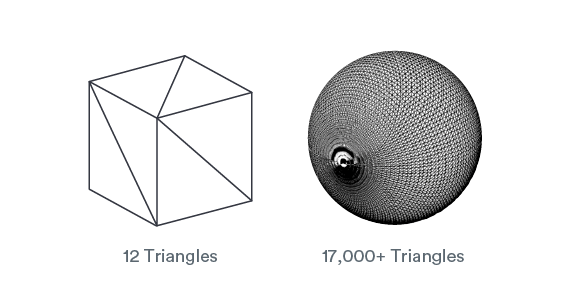
\includegraphics[width=.4\textwidth]{stl_file_1}
	\ccaption{Wireframe eines Würfels und einer Kugel im STL-Datenformat}{\url{https://www.protolabs.com/media/1022944/pl-dt-may-2021_570x308-02.png}}
	\label{img:stl_1}
\end{center}
\end{figure}	

Die Grundlage eines jeden 3D-gedruckten Modells ist immer ein Computer-Assisted-Design-Modell (CAD), welches das gewünschte Teil durch 2D-Zeichnungen darstellt, welche danach zu Körpern extrudiert werden mit verschiedenen Tools. Diese Modelle werden nun in Standard-Tesselation-Language-Datei (STL) konvertiert, um sie für den Slicer, ein Programm, dass das Modell für den Drucker konvertiert, verständlich ist. Eine STL-Datei stellt das Modell als eine Punktwolke dar, wobei immer 3 Punkte ein Dreieck bilden. Ein weiterer gespeichterter Aspekt ist die Normalrichtung eines jeden Dreiecks, damit der Slicer damit berechnen kann, welche Seite die Äußere ist. 

Dieses Konzept ist sehr effizient darin, ebene Oberflächen darzustellen wie Rechtecke, da diese nur aus 2 Dreiecken bestehen. Wenn eine Krümmung einzurechnen ist, muss wie in Abb. \ref{img:stl_1} zu erkennen ist, diese Krümmung mit Dreiecken annähernd dargestellt werden. Dieser Vorgang führt immer eine Ungenauigkeit ein. Diese liegt im Durchschnitt bei in etwa $\qty{0.05}{\centi\metre}$ oder einer aufgetragenen Schicht des handelsüblichen Geräts. Diese Problematik kann durch höhere Auflösung reduziert werden, da die meisten CAD-Suites einen Approximationsgrad angeben lassen, aber als Konsequenz sind die resultierende enorme Dateigröße sowie auch der stark ansteigende Rechenaufwand zu beachten. \parencite{ADOBLESTL} 

Als Alternative zum STL-Format steht das STEP-Format, welches Krümmungen mit sogenannten Non-Uniform Rational B-Splines (NURBS) darstellt.
Diese ermöglichen es, beliebige Kurven und Formen darzustellen. Das Format wird immer beliebter, wobei es noch weit  vom Nutzungsgrad der STL-Dateien entfernt ist. \parencite{ADOBESTEP}


\end{document}
